\documentclass[a4paper,12pt,twoside]{memoir}

% Castellano
\usepackage[spanish,es-tabla]{babel}
\selectlanguage{spanish}
\usepackage[utf8]{inputenc}
\usepackage[T1]{fontenc}
\usepackage{lmodern} % Scalable font
\usepackage{microtype}
\usepackage{placeins}
% Añado paquete para poder añadir TODO's
\usepackage{todonotes}

\RequirePackage{booktabs}
\RequirePackage[table]{xcolor}
\RequirePackage{xtab}
\RequirePackage{multirow}

% Añado listings para ver el código en la memoria mejor
\usepackage{listings}

% Definir colores personalizados
\lstset{
	basicstyle=\ttfamily\footnotesize,  % Estilo básico del texto
	keywordstyle=\color{blue},          % Estilo de las palabras clave
	commentstyle=\color{green},         % Estilo de los comentarios
	stringstyle=\color{red},            % Estilo de las cadenas
	numbers=left,                       % Números de línea en la izquierda
	numberstyle=\tiny\color{gray},      % Estilo de los números de línea
	stepnumber=1,                       % Cada línea numerada
	frame=single,                       % Cuadro alrededor del código
	breaklines=true,                    % Romper líneas largas
	captionpos=b,                       % Posición del caption (debajo)
	tabsize=2,                          % Tamaño de tabulación
	showspaces=false,                   % No mostrar espacios
	showstringspaces=false,             % No mostrar espacios en las cadenas
	showtabs=false,                     % No mostrar tabulaciones
	language=Python                     % Se usa el estilo de Python como base
}

\renewcommand\lstlistlistingname{Índice de Códigos}
\renewcommand\lstlistingname{Código}



% Links
\PassOptionsToPackage{hyphens}{url}\usepackage[colorlinks]{hyperref}
\hypersetup{
	allcolors = {red}
}

% Acrónimos y glosario
\usepackage[acronym]{glossaries}
\makenoidxglossaries
%\usepackage[acronym]{glossaries}
%\makeglossaries

\newacronym{cod}{CoT}{\textit{Cadena de pensamiento}}
\newacronym{crud}{CRUD}{\textit{Create, Read, Update, Delete}}
\newacronym{gui}{GUI}{\textit{{Interfaz Gráfica de Usuario}}}
\newacronym{ia}{IA}{\textit{{Inteligencia Artificial}}}
\newacronym{ide}{IDE}{\textit{{Entorno de Desarrollo Integrado}}}
\newacronym{llm}{LLM}{\textit{Modelos de Lenguaje de Gran Escala}}
\newacronym{nlp}{NLP}{\textit{Procesamiento del Lenguaje Natural}}
\newacronym{odm}{ODM}{\textit{Objetivos de Desarrollo del Milenio}}
\newacronym{ods}{ODS}{\textit{Objetivos de Desarrollo Sostenible}}
\newacronym{onu}{ONU}{\textit{Organización de las Naciones Unidas}}
\newacronym{osm}{OSM}{\textit{{Open Street Maps}}}
\newacronym{osrm}{OSRM}{\textit{{Open Source Routing Machine}}}
\newacronym{pdi}{PDI}{\textit{Puntos de Interés}}
\newacronym{rag}{RAG}{\textit{Retrieval Augmented Generation}}
\newacronym{sc}{Smart City}{\textit{Ciudades Inteligentes}}
\newacronym{sdg}{SDG}{\textit{Sustainable Development Goals}}
\newacronym{sdg11}{SDG11}{\textit{Sustainable Cities and Communities}}
\newacronym{sica}{SICA}{\textit{{Sistema de Información sobre Contaminación Acústica}}}
\newacronym{sig}{GIS}{\textit{Sistemas de Información Geográfica}}
\newacronym{tfg}{TFG}{\textit{Trabajo de Fin de Grado}}


% Acrónimos en inglés
\newacronym{llme}{LLM}{\textit{Large Language Models}}
\newacronym{gis}{SIG}{\textit{Geographic Information Systems}}
\newacronym{poie}{POI}{\textit{Points of Interest}}

% Glosario
\newglossaryentry{ingenieria_prompt}
{
	name=Ingeniería del prompt,
	description={Proceso de optimización y diseño de instrucciones (prompts) para mejorar las respuestas de los modelos de lenguaje a gran escala (LLM)}
}
\newglossaryentry{zero-shot}{
	name={Zero-shot learning},
	description={Técnica en la que el modelo no recibe ejemplos previos sobre cómo realizar una tarea. El modelo interpreta la solicitud basado únicamente en el contexto.}
}

\newglossaryentry{few-shot}{
	name={Few-shot learning},
	description={Técnica en la que el modelo recibe algunos ejemplos en el prompt para comprender con mayor precisión lo que se espera.}
}

\newglossaryentry{tool-calling}{
	name={Tool calling (Function calling)},
	description={Técnica que garantiza que el modelo genere una salida en un formato estructurado y procesable, como JSON.}
}

\newglossaryentry{rag_glos}{
	name={RAG},
	description={\textit{Generación Aumentada por Recuperación}, técnica en la que un modelo LLM se nutre de información adicional para mejorar sus respuestas}
}

\newglossaryentry{agentes}{
	name={Agentes},
	description={Herramientas que alimentan a un LLM con información adicional obtenida de diversas fuentes como bases de datos, motores de búsqueda o páginas web}
}

\newglossaryentry{tokenizacion}{
	name={Tokenización},
	description={Proceso de dividir una cadena de texto en elementos más pequeños (tokens) para que sean procesados por un modelo de lenguaje}
}

\newglossaryentry{embeddings}{
	name={Embeddings},
	description={Técnica que convierte información en vectores numéricos de n dimensiones, utilizados por los modelos LLM para representar datos en un espacio vectorial}
}

\newglossaryentry{zero_shot}{
	name={Zero-shot learning},
	description={Técnica en la que el LLM realiza una tarea sin recibir ejemplos previos, basándose únicamente en su entrenamiento y contexto}
}

\newglossaryentry{few_shot}{
	name={Few-shot learning},
	description={Técnica en la que se proporcionan al modelo algunos ejemplos de la tarea que se quiere realizar, para mejorar la precisión de la respuesta}
}

\newglossaryentry{tool_calling}{
	name={Tool calling},
	description={Método utilizado para generar salidas precisas en formatos específicos, como JSON, facilitando la integración del LLM en aplicaciones}
}




% Ecuaciones
\usepackage{amsmath}

% Rutas de fichero / paquete
\newcommand{\ruta}[1]{{\sffamily #1}}

% Párrafos
\nonzeroparskip

% Huérfanas y viudas
\widowpenalty100000
\clubpenalty100000

% Imágenes

% Comando para insertar una imagen en un lugar concreto.
% Los parámetros son:
% 1 --> Ruta absoluta/relativa de la figura
% 2 --> Texto a pie de figura
% 3 --> Tamaño en tanto por uno relativo al ancho de página
\usepackage{graphicx}
\newcommand{\imagen}[3]{
	\begin{figure}[!h]
		\centering
		\includegraphics[width=#3\textwidth]{#1}
		\caption{#2}\label{fig:#1}
	\end{figure}
	\FloatBarrier
}

% Comando para insertar una imagen sin posición.
% Los parámetros son:
% 1 --> Ruta absoluta/relativa de la figura
% 2 --> Texto a pie de figura
% 3 --> Tamaño en tanto por uno relativo al ancho de página
\newcommand{\imagenflotante}[3]{
	\begin{figure}
		\centering
		\includegraphics[width=#3\textwidth]{#1}
		\caption{#2}\label{fig:#1}
	\end{figure}
}

% El comando \figura nos permite insertar figuras comodamente, y utilizando
% siempre el mismo formato. Los parametros son:
% 1 --> Porcentaje del ancho de página que ocupará la figura (de 0 a 1)
% 2 --> Fichero de la imagen
% 3 --> Texto a pie de imagen
% 4 --> Etiqueta (label) para referencias
% 5 --> Opciones que queramos pasarle al \includegraphics
% 6 --> Opciones de posicionamiento a pasarle a \begin{figure}
\newcommand{\figuraConPosicion}[6]{%
  \setlength{\anchoFloat}{#1\textwidth}%
  \addtolength{\anchoFloat}{-4\fboxsep}%
  \setlength{\anchoFigura}{\anchoFloat}%
  \begin{figure}[#6]
    \begin{center}%
      \Ovalbox{%
        \begin{minipage}{\anchoFloat}%
          \begin{center}%
            \includegraphics[width=\anchoFigura,#5]{#2}%
            \caption{#3}%
            \label{#4}%
          \end{center}%
        \end{minipage}
      }%
    \end{center}%
  \end{figure}%
}

%
% Comando para incluir imágenes en formato apaisado (sin marco).
\newcommand{\figuraApaisadaSinMarco}[5]{%
  \begin{figure}%
    \begin{center}%
    \includegraphics[angle=90,height=#1\textheight,#5]{#2}%
    \caption{#3}%
    \label{#4}%
    \end{center}%
  \end{figure}%
}
% Para las tablas
\newcommand{\otoprule}{\midrule [\heavyrulewidth]}
%
% Nuevo comando para tablas pequeñas (menos de una página).
\newcommand{\tablaSmall}[5]{%
 \begin{table}
  \begin{center}
   \rowcolors {2}{gray!35}{}
   \begin{tabular}{#2}
    \toprule
    #4
    \otoprule
    #5
    \bottomrule
   \end{tabular}
   \caption{#1}
   \label{tabla:#3}
  \end{center}
 \end{table}
}

%
% Nuevo comando para tablas pequeñas (menos de una página).
\newcommand{\tablaSmallSinColores}[5]{%
 \begin{table}[H]
  \begin{center}
   \begin{tabular}{#2}
    \toprule
    #4
    \otoprule
    #5
    \bottomrule
   \end{tabular}
   \caption{#1}
   \label{tabla:#3}
  \end{center}
 \end{table}
}

\newcommand{\tablaApaisadaSmall}[5]{%
\begin{landscape}
  \begin{table}
   \begin{center}
    \rowcolors {2}{gray!35}{}
    \begin{tabular}{#2}
     \toprule
     #4
     \otoprule
     #5
     \bottomrule
    \end{tabular}
    \caption{#1}
    \label{tabla:#3}
   \end{center}
  \end{table}
\end{landscape}
}

%
% Nuevo comando para tablas grandes con cabecera y filas alternas coloreadas en gris.
\newcommand{\tabla}[6]{%
  \begin{center}
    \tablefirsthead{
      \toprule
      #5
      \otoprule
    }
    \tablehead{
      \multicolumn{#3}{l}{\small\sl continúa desde la página anterior}\\
      \toprule
      #5
      \otoprule
    }
    \tabletail{
      \hline
      \multicolumn{#3}{r}{\small\sl continúa en la página siguiente}\\
    }
    \tablelasttail{
      \hline
    }
    \bottomcaption{#1}
    \rowcolors {2}{gray!35}{}
    \begin{xtabular}{#2}
      #6
      \bottomrule
    \end{xtabular}
    \label{tabla:#4}
  \end{center}
}

%
% Nuevo comando para tablas grandes con cabecera.
\newcommand{\tablaSinColores}[6]{%
  \begin{center}
    \tablefirsthead{
      \toprule
      #5
      \otoprule
    }
    \tablehead{
      \multicolumn{#3}{l}{\small\sl continúa desde la página anterior}\\
      \toprule
      #5
      \otoprule
    }
    \tabletail{
      \hline
      \multicolumn{#3}{r}{\small\sl continúa en la página siguiente}\\
    }
    \tablelasttail{
      \hline
    }
    \bottomcaption{#1}
    \begin{xtabular}{#2}
      #6
      \bottomrule
    \end{xtabular}
    \label{tabla:#4}
  \end{center}
}

%
% Nuevo comando para tablas grandes sin cabecera.
\newcommand{\tablaSinCabecera}[5]{%
  \begin{center}
    \tablefirsthead{
      \toprule
    }
    \tablehead{
      \multicolumn{#3}{l}{\small\sl continúa desde la página anterior}\\
      \hline
    }
    \tabletail{
      \hline
      \multicolumn{#3}{r}{\small\sl continúa en la página siguiente}\\
    }
    \tablelasttail{
      \hline
    }
    \bottomcaption{#1}
  \begin{xtabular}{#2}
    #5
   \bottomrule
  \end{xtabular}
  \label{tabla:#4}
  \end{center}
}



\definecolor{cgoLight}{HTML}{EEEEEE}
\definecolor{cgoExtralight}{HTML}{FFFFFF}

%
% Nuevo comando para tablas grandes sin cabecera.
\newcommand{\tablaSinCabeceraConBandas}[5]{%
  \begin{center}
    \tablefirsthead{
      \toprule
    }
    \tablehead{
      \multicolumn{#3}{l}{\small\sl continúa desde la página anterior}\\
      \hline
    }
    \tabletail{
      \hline
      \multicolumn{#3}{r}{\small\sl continúa en la página siguiente}\\
    }
    \tablelasttail{
      \hline
    }
    \bottomcaption{#1}
    \rowcolors[]{1}{cgoExtralight}{cgoLight}

  \begin{xtabular}{#2}
    #5
   \bottomrule
  \end{xtabular}
  \label{tabla:#4}
  \end{center}
}



\graphicspath{ {./img/} }

% Capítulos
\chapterstyle{bianchi}
\newcommand{\capitulo}[2]{
	\setcounter{chapter}{#1}
	\setcounter{section}{0}
	\setcounter{figure}{0}
	\setcounter{table}{0}
	\chapter*{\thechapter.\enskip #2}
	\addcontentsline{toc}{chapter}{\thechapter.\enskip #2}
	\markboth{#2}{#2}
}

% Apéndices
\renewcommand{\appendixname}{Apéndice}
\renewcommand*\cftappendixname{\appendixname}

\newcommand{\apendice}[1]{
	%\renewcommand{\thechapter}{A}
	\chapter{#1}
}

\renewcommand*\cftappendixname{\appendixname\ }

% Formato de portada
\makeatletter
\usepackage{xcolor}
\newcommand{\tutor}[1]{\def\@tutor{#1}}
\newcommand{\course}[1]{\def\@course{#1}}
\definecolor{cpardoBox}{HTML}{E6E6FF}
\def\maketitle{
  \null
  \thispagestyle{empty}
  % Cabecera ----------------
\noindent
\includegraphics[width=\textwidth]{cabecera}\vspace{1cm}%
  \vfill
  
  % Título proyecto y escudo informática ----------------
  \colorbox{cpardoBox}{%
    \begin{minipage}{.8\textwidth}
      \vspace{.5cm}\Large
      \begin{center}
      \textbf{TFG del Grado en Ingeniería Informática}\vspace{.6cm}\\
      \textbf{\LARGE\@title{}}
      \end{center}
      \vspace{.2cm}
    \end{minipage}

  }%
  \hfill\begin{minipage}{.20\textwidth}
    
\includegraphics[width=\textwidth]{escudoInfor}
  \end{minipage}
  \vfill
  
  % Datos de alumno, curso y tutores ------------------
  \begin{center}%
  {%
    \noindent\LARGE
    Presentado por \@author{}\\ 
    en Universidad de Burgos --- \@date{}\\
    Tutor: \@tutor{}\\
  }%
  \end{center}%
  \null
  \cleardoublepage
  }
\makeatother

\newcommand{\nombre}{Fernando Pisot Serrano}


% Datos de portada
\title{\fontsize{18pt}{22pt}\selectfont Eco City Tours\\
	\fontsize{16pt}{18pt}\selectfont Aplicación móvil para la generación de rutas turísticas sostenibles propuestas por modelos de lenguaje de gran escala}
\author{\nombre}
\tutor{Carlos López Nozal}
\date{\today}

\begin{document}

\maketitle


%\newpage\null\thispagestyle{empty}\newpage


%%%%%%%%%%%%%%%%%%%%%%%%%%%%%%%%%%%%%%%%%%%%%%%%%%%%%%%%%%%%%%%%%%%%%%%%%%%%%%%%%%%%%%%%
\thispagestyle{empty}


\noindent
\includegraphics[width=\textwidth]{cabecera}\vspace{1cm}

\noindent D. Carlos López Nozal, profesor del departamento de Ingeniería Informática, área de Lenguajes y Sistemas Informáticos.

\noindent Expone:

\noindent Que el alumno D. \nombre, con DNI 70873328R, ha realizado el Trabajo final de Grado en Ingeniería Informática. 

\noindent Y que dicho trabajo ha sido realizado por el alumno bajo la dirección del que suscribe, en virtud de lo cual se autoriza su presentación y defensa.

\begin{center} %\large
En Burgos, {\large \today}
\end{center}

\vfill\vfill\vfill

\begin{center}
  Vº. Bº. del Tutor:\\[2cm]
  D. Carlos López Nozal \@tutor{}
  \end{center}


\newpage\null\thispagestyle{empty}\newpage




\frontmatter

% Abstract en castellano
\renewcommand*\abstractname{Resumen}
\begin{abstract}
Eco City Tours es una aplicación móvil desarrollada con Flutter que propone al usuario rutas turísticas sostenibles. La aplicación se enfoca en la promoción de rutas no motorizadas, optimizadas para ciclistas y peatones, que conectan lugares de interés con el objetivo de fomentar la movilidad sostenible. Las rutas se generan con tecnologías usando \acrfull{gis}. Los \acrfull{pdi} se enriquecen con información detallada sobre lugares turísticos mediante inteligencia artificial consultando en lenguaje natural a \acrfull{llm}.

Esta aplicación se alinea con el concepto de \acrshort{sc}, promoviendo activamente los \acrfull{ods}, con un enfoque particular en el ODS11 (Ciudades y Comunidades Sostenibles).


\end{abstract}

\renewcommand*\abstractname{Descriptores}
\begin{abstract}
Movilidad Sostenible, ODS, LLM, Smart City, Flutter.
\end{abstract}

\clearpage

% Abstract en inglés
\renewcommand*\abstractname{Abstract}
\begin{abstract}
	Eco City Tours is a mobile application \textbf{developed with Flutter} that suggests tourist routes to users. The application focuses on promoting non-motorized routes, optimized for cyclists and pedestrians, connecting points of interest with the goal of fostering sustainable mobility. The routes are generated using technologies based on \acrfull{sig}. The \acrfull{poie} are enriched with detailed information about tourist spots through artificial intelligence, consulting \acrfull{llme} via natural language queries.
	
	This application aligns with the concept of \acrshort{sc}, actively promoting the \acrfull{sdg}, with a particular focus on the SDG11 (Sustainable Cities and Communities).
\end{abstract}

\renewcommand*\abstractname{Keywords}
\begin{abstract}
	Sustainable Mobility, SDGs, LLM, Smart City, Flutter.
\end{abstract}



\clearpage

% Indices
\tableofcontents

\clearpage

\listoffigures

\clearpage

\listoftables
\clearpage

\lstlistoflistings
\clearpage

\mainmatter
\capitulo{1}{Introducción}

El crecimiento de población en las ciudades \cite{nieuwenhuijsen_urban_2020} y el turismo como catalizador de la gentrificación supone el gran campo de batalla para gobiernos locales de los países occidentales que han visto como la falta de una legislación controlada del turismo supone un grave problema afectando múltiples niveles de la convivencia, economía y el medio ambiente. A pesar de los avances en la promoción de un nuevo modelo urbano, muchas urbes aún enfrentan desafíos significativos en la integración de prácticas sostenibles en la vida cotidiana de sus habitantes. La falta de información accesible y personalizada sobre rutas y actividades que promuevan la movilidad sostenible y el turismo responsable es un marco común que se debe desarrollar si se quiere evitar que el conflicto crezca sin fin. Esta brecha de información impide que tanto residentes como turistas adopten hábitos más sostenibles que beneficien a la comunidad local y al medio ambiente en un marco global.

Fomentar el Turismo Sostenible supone una gran oportunidad para intentar contrarrestar la deriva actual. Y es que el turismo es un motor fundamental de la economía a nivel global y por tanto tiene la capacidad de transformarse para ayudar a la sostenibilidad del planeta.  Destaca en este marco de trabajo el  objetivo \acrshort{ods} número 11 titulado \textit{Ciudades y Comunidades Sostenibles}. Según el informe de la \textit{UNESCO}, \cite{ionescu_progress_2024}, no solo es crucial por sí mismo, sino que actúa como un factor multiplicador, influyendo indirectamente en la consecución de otros \acrshort{ods} debido a su enfoque integral y transversal.

Eco City Tours \textbf{aúna estos esfuerzos al proporcionar una herramienta práctica y accesible} para la promoción del ODS11 y la movilidad sostenible. La aplicación ha sido desarrollada en Flutter y utiliza \acrfull{llm} para generar rutas turísticas personalizadas que conecten \acrlong{pdi}. La aplicación se enfoca en las \textbf{preferencias del usuario}, ofreciendo \textbf{rutas optimizadas} para ciclistas y peatones promoviendo así la movilidad sostenible.

Las preferencias del usuario se comunicarán al modelo a través de un menú, donde éste podrá elegir qué lugar visitar, si realizar el tour a pie o en bicicleta, cuántos \acrlong{pdi} incluir en la ruta y sus gustos a la hora de viajar. El sistema generará el camino más corto, calculado entre los distintos \acrshort{pdi} a visitar, usando para ello un servicio de geolocalización.

Mientras que muchas de las aplicaciones similares revisadas solo utilizan información comercial para definir rutas turísticas, Eco City Tours solicita que se tengan en cuenta prácticas sostenibles como la deslocalización del turismo a la hora de elegir destinos. Todas estas consideraciones enriquecen la experiencia turística de los visitantes \cite{mitas_tell_2023}, e incluso promueven el crecimiento económico de las comunidades locales. De este modo, Eco City Tours logra un impacto positivo tanto a nivel local como global.
\capitulo{2}{Objetivos del proyecto}

\section{Objetivos funcionales}

Estos objetivos se centran en las funcionalidades y características que debe tener la aplicación Eco City Tours para satisfacer las necesidades y expectativas de los usuarios. A continuación se detallan los objetivos funcionales del proyecto:

\begin{itemize}
    \item \textbf{Propuesta de rutas turísticas personalizadas}: La aplicación debe ser capaz de generar rutas turísticas personalizadas basadas en las preferencias del visitante utilizando \acrfull{llm}. Para llevarlo a cabo, el usuario facilitará al modelo sus preferencias, eligiendo entre otras opciones el medio de transporte elegido o el número de \acrfull{pdi} a visitar.
    \item \textbf{Obtener los \acrfull{pdi}}: A través de la interacción con el modelo, la aplicación le indicará que debe priorizar un \acrshort{pdi} sobre otro en función de criterios sostenibles como la deslocalización del turismo y preferencias de usuario como puedan ser duración de la visita o medio de transporte ecológico a utilizar.
    \item \textbf{Visualización de rutas en mapa}: La aplicación debe mostrar las rutas sugeridas en un mapa utilizando herramientas \acrshort{sig}.
    \item \textbf{Optimización para ciclistas y peatones}: la aplicación usará un servicio de navegación de calidad que debe ser capaz de calcular rutas seguras para peatones y priorizar carriles bicis sobre carreteras compartidas con vehículos motorizados.
    \item \textbf{Gestión de rutas}: La aplicación permitirá a los usuarios crear, guardar y compartir rutas turísticas, facilitando una mayor personalización y aprovechamiento de la experiencia turística.
    

\end{itemize}

\section{Objetivos no funcionales}

Los objetivos no funcionales se refieren a los desafíos y metas que se deben abordar para desarrollar el software. Estos objetivos abarcan aspectos como la arquitectura del sistema, las tecnologías a utilizar y las metodologías de desarrollo. A continuación se detallan los objetivos no funcionales del proyecto:

\begin{itemize}
	\item \textbf{Integración de inteligencia artificial usando \acrfull{nlp}}: La aplicación contará con un modelo de lenguaje preseleccionado, que facilita la propuesta de rutas turísticas personalizadas y la obtención de información relevante de \acrlong{pdi}. Esta elección garantiza la estabilidad y el rendimiento de la aplicación, proporcionando información precisa y relevante sin la necesidad de cambiar modelos, lo cual reduce la complejidad de mantenimiento.
    \item \textbf{Uso de Herramientas Open-Source}: se priorizará para el desarrollo de la aplicación programas, paquetes, servicios o librerías que sean de código abierto, siempre que sea posible y no repercuta en la calidad del producto final. Se priorizará en todo caso una solución que no incurra en gasto alguno para el desarrollador o al usuario final por su uso. De esta manera se intenta fomentar el \acrshort{ods} 4: \textit{Educación de calidad} que busca garantizar una educación inclusiva, equitativa y de calidad y promover oportunidades de aprendizaje para todos.
    \item \textbf{Usabilidad}: la interacción del usuario con la aplicación debe ser intuitiva y sencilla, permitiendo un rápido aprendizaje de todas sus funcionalidades. El diseño de la interfaz debe estar orientado a ofrecer una experiencia de uso fluida. 
\end{itemize}

\section{Objetivos personales}


\begin{itemize}
	\item \textbf{Formación en \acrshort{llm} y su integración en aplicaciones software.} Dada la rápida evolución de los \acrfull{llm} y la amplitud de campos del conocimiento en los que se pueden utilizar, obtener una base de conocimientos destacable en este área sería un objetivo que me permitiría expandir mi futuro académico y por tanto distinguir mi perfil profesional especializándome en un sector con fuerte expansión.
	\item \textbf{Desarrollo de aplicación móvil profesional}: poner en práctica lo aprendido en varios cursos de auto-formación online en \textbf{Dart y Flutter.} La aplicación de este proyecto puede ser parte de mi porfolio con aplicaciones que muestren mis habilidades a futuros empleadores.
	\item \textbf{Finalización del \acrshort{tfg} y Grado}: tras no haber completado la Ingeniería Técnica Informática en su momento por no haber realizado el Proyecto Fin de Carrera, la realización de este \acrshort{tfg} marca la culminación de mi formación académica como ingeniero.
\end{itemize}

\capitulo{3}{Conceptos teóricos}

En este capítulo se describen los conceptos necesarios para comprender el funcionamiento de la aplicación desarrollada.

\section{Sistemas de Información Geográfica (SIG)}
	Un Sistema de Información Geográfica, comúnmente abreviado como \acrshort{sig} o \acrshort{gis}, es cualquier herramienta hardware o software que permita la realización de tareas sobre información que esté georreferenciada, es decir que los datos incluyen una ubicación en coordenadas geográficas.~\cite{qgis_introduction_gis}
	Estas herramientas están específicamente diseñadas para trabajar con datos que no solo realizan operaciones usuales de inserción, eliminación, actualización y extracción en una base de datos común (\acrshort{crud}), sino que realizan análisis con respecto a la ubicación o características geoespaciales o topográficas. Junto con los análisis espaciales, proporciona una mejor visualización de los datos con mapas, de modo que uno pueda presentar la información efectivamente en una manera legible que de otro modo sería difícil de interpretar.
	 
	Estas herramientas están cada vez más presentes en diversos campos de la ciencia y la informática. Facilitan la toma de decisiones en áreas como el desarrollo urbano o la optimización de rutas. Además, son capaces de mejorar la gestión de empresas que ofrecen servicios descentralizados, como el suministro de agua o energía. Es por ello que su aplicación es clave también en el análisis del cambio climático y otros desafíos globales como los \acrlong{ods}.
	
	\subsection{Servicios GIS empleados en Eco City Tours}
	Los sistemas o herramientas con referencias geográficas son comúnmente utilizadas como servicios en el desarrollo de aplicaciones con componentes de información geográfica. Los proveedores de estos servicios facilitan datos georreferenciados según las peticiones del usuario. Eco City Tours utiliza varios servicios GIS para su funcionamiento. Entre ellos se incluyen:
	\begin{itemize}
		\item \textbf{Servicio de mapas}: con Google como proveedor~\cite{google_maps} se usa este servicio para proveer a la aplicación de un mapa para mostrar de fondo así como marcadores y polilíneas de rutas.
		
		\item \textbf{Geocodificación}: sirve para obtener las coordenadas GPS de un \acrlong{pdi} o conseguir el nombre de un lugar próximo a unas coordenadas dadas (inverse geocoding). Se ha utilizado este servicio con el proveedor MapBox.\cite{mapbox_geocoding}
		
		\item \textbf{Servicio de navegación y de optimización de rutas}: el servicio de navegación \cite{mapbox_directions} nos proporciona una ruta entre dos \acrlong{pdi} y el servicio de optimización permite generar una ruta que sea la más corta entre múltiples \acrshort{pdi} en el mapa. El proveedor de este servicio es MapBox \cite{mapbox_optimization}.De esta manera se soluciona este problema popularmente conocido como \textit{el problema del viajante}\cite{ubu_algoritmia} dando el recorrido más corto posible para el medio de transporte elegido en la petición al servicio.
		
	\end{itemize}
	
\section{Objetivos de Desarrollo Sostenible (ODS)}
	Los \acrlong{ods} son una lista de 17 objetivos globales adoptados por la Asamblea General de la \acrfull{onu} el 25 de septiembre de 2015, como parte de la Agenda 2030 para el Desarrollo Sostenible. Según la \acrshort{onu} ~\cite{un_sustainable_development}, ``\textit{los líderes mundiales adoptaron un conjunto de objetivos globales para erradicar la pobreza, proteger el planeta y asegurar la prosperidad para todos como parte de una nueva agenda de desarrollo sostenible. Cada objetivo tiene metas específicas que deben alcanzarse en los próximos 15 años}''.		
	\imagen{odss}{Objetivos de Desarrollo Sostenible}{1}
	Los \acrshort{ods} suceden a los \acrfull{odm}, que fueron formulados en el año 2000 y finalizados en 2015. A diferencia de los \acrshort{odm}, que se enfocaban principalmente en los países en desarrollo, los \acrshort{ods} son universales y están diseñados para ser aplicados por todos los países, sin importar su nivel de desarrollo. Los \acrlong{ods} son la incorporación de los tres pilares del desarrollo sostenible: económico, social y ambiental, están definidos por una perspectiva universal e indivisible que tiene en cuenta las relaciones entre los tres ámbitos.
		
	Los 17 ODS son un conjunto integral que abarca desafíos globales que afectan a la humanidad y el planeta (Ver Fig. \ref{fig:odss}). Cada objetivo se desglosa en metas específicas y medibles. Algunos de los objetivos más relevantes para el marco de sostenibilidad y desarrollo urbano son los siguientes:
	\begin{itemize}
		\item \textbf{ODS 11}: \textit{Ciudades y comunidades sostenibles}: Busca hacer que las ciudades y los asentamientos humanos sean inclusivos, seguros, resilientes y sostenibles. Dado que más del 55\% de la población mundial vive en áreas urbanas, este objetivo es crucial para mejorar la calidad de vida y reducir el impacto ambiental en las ciudades. Incluye metas como el acceso a una vivienda adecuada y asequible, el transporte sostenible, la planificación urbana inclusiva y la reducción del impacto ambiental urbano.
		
		\item \textbf{ODS 13}: \textit{Acción por el clima}: Llama a tomar medidas urgentes para combatir el cambio climático y sus impactos, incluyendo la mitigación de emisiones de gases de efecto invernadero y la adaptación a los efectos adversos del cambio climático.
		
		\item \textbf{ODS 7}: \textit{Energía asequible y no contaminante}: Promueve el acceso universal a energía moderna, asequible, confiable y sostenible, lo que implica la expansión de las energías renovables y la mejora en la eficiencia energética. Este objetivo es clave para reducir las emisiones de carbono y combatir el cambio climático.
		
	\end{itemize}
	
	\subsection{ODS y tecnología GIS en la planificación urbana}
	El uso de tecnologías como los Sistemas de Información Geográfica (GIS) desempeña un papel crucial en la implementación y seguimiento de los ODS, especialmente en el ámbito urbano. Los GIS permiten en el campo de la planificación urbana:
	\begin{itemize}
		\item \textbf{Monitorización del desarrollo urbano}: Ayudan a analizar cómo crecen las ciudades y qué impacto tienen en el medio ambiente, lo cual es vital para cumplir con las metas de ciudades sostenibles.
		
		\item \textbf{Optimización de rutas sostenibles}: Facilitan la creación de rutas para peatones y ciclistas que minimicen el uso de vehículos motorizados, contribuyendo a la reducción de emisiones de gases de efecto invernadero.
		
		\item \textbf{Evaluación de riesgos ambientales}: Permiten identificar áreas vulnerables a riesgos naturales, como inundaciones o deslizamientos de tierra, y planificar medidas de adaptación al cambio climático.
		
		\item \textbf{Gestión de la masificación turística}: Herramientas diagnósticas como el \acrfull{sica}, una plataforma dependiente del Ministerio de Transportes, Movilidad y Agenda Urbana \cite{sica_mapa_ruido}, pueden ayudar a identificar zonas de masificación turística. Al combinar estos datos con otras fuentes de datos como la ubicación de personas a través de sus dispositivos móviles, es posible diseñar alternativas o implementar restricciones que redistribuyan el flujo de turistas, minimizando su impacto negativo en el entorno local.
 
		
	\end{itemize}
	

\section{Modelos de lenguaje a gran escala (LLM)}
Los modelos de lenguaje a gran escala son un tipo de inteligencia artificial que ha sido entrenada para realizar tareas de \acrfull{nlp}. Estas inteligencias artificiales son entrenadas con ingentes cantidades de datos que los hacen capaces de comprender peticiones y responder a las éstas en los mismos términos de lenguaje generando una comunicación entre el usuario y la máquina.
	
	\subsection{Técnicas de \gls{ingenieria_prompt}}
	En el desarrollo de este \acrshort{tfg}, se han implementado y evaluado diversas técnicas de \gls{ingenieria_prompt} con el fin de mejorar la interacción y los resultados generados por los \acrshort{llm}. A continuación, se detallan las principales técnicas empleadas durante este proceso. Para obtener más información sobre estas técnicas y otras estrategias de \gls{ingenieria_prompt}, se puede consultar la guía disponible en \href{https://www.promptingguide.ai/es}{Prompting Guide}\cite{promptingguide}.
	
	\gls{zero-shot} se trata de una técnica en la que el usuario no facilita al modelo ningún ejemplo de cómo realizar una tarea. El \acrshort{llm} por tanto interpreta basado en el contexto y su propio entrenamiento lo que se ha requerido y responde acorde a estos datos. Esta técnica se usa cuando lo que se prioriza es la rapidez del modelo frente a la precisión de la salida aportada. Cuando se requiere una mayor exactitud en la interacción, es recomendable emplear la técnica de \gls{few-shot}, que consiste en proporcionar al modelo algunos ejemplos en el prompt para guiarlo hacia una respuesta mejorada según el criterio del desarrollador.
	
	Una vez que se logra establecer el formato de las respuestas, es importante asegurar que el modelo sea capaz de interactuar con herramientas externas o APIs. Aquí es donde entra en juego la técnica de \gls{tool-calling}.
	Se trata de una habilidad clave para construir chatbots o agentes potenciados por \acrshort{llm} que necesitan recuperar contexto o interactuar con herramientas externas convirtiendo \acrlong{nlp} en llamadas a APIs.
	Este enfoque de \gls{tool-calling} \textbf{permite una mejora en la modularidad del proyecto}. Al separar el nivel de abstracción, permite por ejemplo cambiar el modelo \acrshort{llm} de origen sin afectar al funcionamiento general del sistema, ya que la estructura de la salida permanece constante.

	A continuación, se ilustra un ejemplo de cómo se nutre al modelo con una plantilla que sirve de estructura para la respuesta, obteniendo de manera consistente datos en formato JSON. Este ejemplo se puede encontrar en el \href{https://github.com/fps1001/TFGII_FPisot/tree/main/project-prototypes/prompting.ipynb}{prototipo Python} del proyecto: 
	
	\begin{lstlisting}[language=Python, caption={Ejemplo de uso de \textit{few-shot} y \textit{tool-calling} para obtener puntos de interés turísticos}]
		# Un ejemplo de respuesta que queremos obtener seria la siguiente:
		plantilla_salida = """[{
			"nombre": "Sagrada Familia", 
			"gps": "41.4036, 2.1744", 
			"descripcion": "Basilica catolica disenada por Gaudi." 
		},
		{
			"nombre": "Parc Guell", 
			"gps": "41.4145, 2.1527", 
			"descripcion": "Parque disenado por Gaudi."
		}]"""
		
		ciudad = "Salamanca"
		complete_and_print(f"""Tu rol es un guia turistico comprometido con el medio ambiente preocupado por la gentrificacion de las ciudades y el turismo masivo. 
		Dime 3 sitios para visitar en {ciudad}. Quiero que la respuesta consista SOLO en los lugares de interes de este lugar, siguiendo el ejemplo de la {plantilla_salida}. Insisto en que no quiero que me des informacion adicional.""")
		
		# Resultado esperado:
		[{
			"nombre": "Catedral Vieja de Salamanca", 
			"gps": "40.9708, -5.6619", 
			"descripcion": "Edificio gotico del siglo XIII."
		},
		{
			"nombre": "Puente de San Esteban", 
			"gps": "40.9713, -5.6624", 
			"descripcion": "Puente medieval que cruza el rio Tormes."
		},
		{
			"nombre": "Jardines de la Alamedilla", 
			"gps": "40.9694, -5.6632", 
			"descripcion": "Jardin barroco en el corazon de la ciudad."
		}]
	\end{lstlisting}
	
	\subsection{Retrieval-Augmented Generation (RAG)}
	Generación Aumentada por Recuperación o \gls{rag_glos} es una técnica usada en modelos de inteligencia artificial en la cual se obtiene información para nutrir a un \acrlong{llm} que ya ha sido entrenado, de esta manera amplía su conocimiento y es capaz de generar una respuesta más precisa, actualizada y completa.
	
	El problema que subyace en los modelos tradicionales es que una vez alimentados con un conjunto de datos, sufren de un aislamiento del mundo que los rodea. Para prevenir este problema se nutre de información que el usuario facilita siguiendo los siguientes pasos:
	\begin{enumerate}
		\item \textbf{Splitter y \gls{tokenizacion}}: La información proporcionada al modelo se divide en tokens, donde cada modelo tiene un límite máximo de tokens que puede procesar como contexto. Además, algunos modelos pueden cobrar al usuario por cada token procesado. Por lo tanto, es fundamental transformar una cadena de texto larga en fragmentos más pequeños y optimizados, utilizando tokens específicos para facilitar la comprensión por parte del modelo. Esta división previa es un paso necesario antes de recuperar la información.
	
		\item \gls{embeddings}: consiste en transformar la información facilitada y representarla en vectores de n dimensiones. Para ello se usa comúnmente otro modelo entrenado para transformar la información en vectores.
		En la imagen \ref{fig:langflow_rag_embeddings_gray} se puede ver cómo la información de Wikipedia API \cite{wikimedia_api} se prepara para guardarse en una base de datos vectorial Astra DB \cite{datastax_astra} para ello usa el modelo Ollama Embeddings
		
		\imagen{langflow_rag_embeddings_gray}{Preparación de la información de un RAG mostrada en la herramienta Langflow}{1}
		
		\item \textbf{RAG}: con la información ampliada ya vectorizada en una base de datos, el usuario genera una entrada o prompt al modelo. Como se ve en la imagen \ref{fig:langflow_rag_retrieval_gray} el \acrshort{llm} OpenAI en este caso selecciona la información más afín de los datos aportados para generar así un prompt ampliado o mejorado que será facilitado al modelo para un procesamiento de información habitual, consiguiendo así un mejor resultado.
		
		\imagen{langflow_rag_retrieval_gray}{Chat Output a través de la salida de un RAG}{1}
	\end{enumerate}
		
	\subsection{Agentes}
	\label{sec:agentes}
	La información que alimenta a los RAG puede ser un archivo de texto con información general de un tema sin embargo hay veces en los que la información no está físicamente en un archivo y se tiene que obtener a través de \gls{agentes}.
	Estas múltiples herramientas pueden ser vistas como aplicaciones que alimentarán al modelo con un conjunto de herramientas tales como motores de búsqueda, bases de datos, páginas web, etc. Una vez provisto con esta información el modelo es capaz de razonar acerca de las acciones que debe cumplir para obtener el mejor resultado.

	
	\subsection{Uso de LLMs en Eco City Tours}
	En este proyecto, los \acrlong{llm} se han empleado para obtener los \acrfull{pdi} a través de un diálogo interactivo entre la \acrlong{ia} y el usuario, donde este último solicita recomendaciones de lugares enfocados en el turismo sostenible. En la sección de \href{https://github.com/fps1001/TFGII_FPisot/tree/main/project-prototypes/README.md}{prototipos}, además de un prototipo con Langflow, se implementa un cuaderno de Python que evalúa las mejoras en las respuestas aplicando diversas técnicas de prompting\cite{promptingguide}. Inicialmente, el prototipo presenta una conversación básica con respuestas de baja calidad o incluso alucinadas, que progresivamente mejoran al incluir estructuras de datos predefinidas en las respuestas. Este enfoque permite que la aplicación aproveche el aprendizaje, generando recomendaciones más precisas y acordes al código requerido en la aplicación móvil.
	
	En cuanto a los \acrfull{rag}, su mayor utilidad suele encontrarse en la mejora de chatbots empresariales, donde se busca ofrecer una atención al cliente más eficiente y precisa. En el contexto de los prototipos desarrollados para este \acrshort{tfg}, se realizaron pruebas con sistemas \acrshort{rag} que recopilaban información a partir de búsquedas en Internet. Las páginas web resultado de las búsquedas eran después tratadas para, una vez procesada su información,  incluirla en el contexto del prompt, lo que permitía al modelo generar respuestas más completas y actualizadas. Sin embargo, los resultados de estas pruebas revelaron que, aunque el sistema proporciona un contexto enriquecido y relevante, los tiempos de respuesta se incrementan significativamente, lo que podría afectar negativamente la experiencia del usuario. Por esta razón,\textbf{ se decidió no implementar estas herramientas en la versión final de la aplicación}, aunque los prototipos quedan disponibles como experimentos, con el fin de inspirar a otros desarrolladores interesados en explorar esta tecnología.

\section{Agilidad y método SCRUM}
La gestión ágil de proyectos de desarrollo de software tiene como pilares fundamentales la flexibilidad, la colaboración y la entrega continua de valor al cliente\cite{agile_alliance}. La agilidad se basa en la idea de ciclos de trabajo cortos e iterativos denominados \textbf{sprints}, donde se produce software funcional al final de cada iteración.

El Manifiesto Ágil (2001) establece cuatro valores fundamentales:
\begin{itemize}
\item Individuos e interacciones sobre procesos y herramientas.
\item Software funcional sobre documentación exhaustiva.
\item Colaboración con el cliente sobre negociación de contratos.
\item Respuesta ante el cambio sobre seguir un plan.
\end{itemize}

\textbf{SCRUM} es un marco de trabajo ágil que facilita la auto-organización del equipo, promueve la transparencia y mejora la capacidad de adaptación del proyecto.

Este enfoque es particularmente valioso en el desarrollo de Eco City Tours, iterando rápidamente sobre incrementos funcionales de la aplicación, validando con pruebas de usuario con prototipos funcionales y ajustando el desarrollo a las necesidades que surgían durante el proceso. El tutor ha jugado los tres roles definidos en SCRUM: usuario para validar los incrementos funcionales, equipo cuando revisa contenido de las tareas y SCRUM master para ayudar ha aplicar la agilidad. El rol principal del estudiante y autor de trabajo es el de equipo. Ambos participantes se han reunido para:

\begin{itemize}
	\item \textbf{Planificación de Sprint}: consiste en la creación y asignación de tareas que se realizarán durante el período de tiempo en que consiste el sprint. A cada tarea se le asigna unos puntos de historia que reflejan el tiempo planificado para realizar dicha tarea. También se planifican etiquetas e hitos para los que las diferentes tareas ayudan a lograr.
	\item \textbf{Sprint review y sprint retrospective}: después de cada sprint y con la ayuda del tutor del \acrshort{tfg} se evalua el trabajo realizado durante el sprint, se 
	
\end{itemize}

El uso de la metodología ágil y el marco SCRUM fue esencial para el éxito del desarrollo de Eco City Tours. La agilidad permitió una colaboración constante y una entrega continua de valor, mientras que SCRUM proporcionó la estructura necesaria para gestionar eficazmente el trabajo, resolver problemas y optimizar el proceso de desarrollo en cada iteración.
\capitulo{4}{Técnicas y herramientas}

El siguiente capítulo presenta las técnicas y herramientas usadas a lo largo del desarrollo de la aplicación Eco City Tours. Se detallarán los aspectos más destacados de cada una de ellas, justificando el porqué de su utilización sobre otras alternativas si las hubiera. Se ha seguido una división en función de su 


\section{Desarrollo relacionado con LLM}
	\subsection{LM Studio}
	LM Studio \cite{lmstudio_ai} es una aplicación enfocada en el despliegue de modelos de lenguaje. Su principal objetivo es facilitar la experimentación con \acrlong{llm} ofreciendo un entorno completo y que integra funcionalidades en el procesamiento de lenguaje natural.
	Estas son algunas de las más destacadas:
	
	
	\begin{itemize}
		
		\item \textbf{Búsqueda y despliegue de modelos en local}: a través de un buscador intuitivo, los usuarios pueden seleccionar, descargar y desplegar cualquier modelo disponible en plataformas como Hugging Face, facilitando su uso local.
		
		\item \textbf{Servidor local de un el modelo}: LM Studio permite crear un servidor local que gestione peticiones de información. Esto es especialmente útil para automatizar procesos que requieran el procesamiento de lenguaje o la gestión de grandes volúmenes de datos.
		
		\item \textbf{Entrenamiento y ajuste de modelo}: LM Studio simplifica el proceso de fine-tuning o ajuste fino, que consiste en optimizar un modelo pre-entrenado mediante conjuntos de datos específicos y tareas concretas para mejorar su rendimiento. Gracias a su interfaz gráfica, esta tarea se vuelve más accesible para los desarrolladores, eliminando gran parte de la complejidad técnica.
		
		\item \textbf{Optimización y monitorización}: permite observar el rendimiento de los modelos analizando su consumo de GPU, memoria o CPU así como su tiempo de respuesta, lo que permite realizar al usuario ajustes con el fin de mejorar el rendimiento del sistema.
	\end{itemize}
	La experimentación con diferentes modelos para decidir cuál usar en Eco City Tours resultó mucho más rápida y eficiente gracias a esta herramienta, en comparación con el uso inicial de un solo modelo a través de Ollama \cite{ollama}.
		
	\subsection{LangFlow}
	LangFlow es una herramienta de código abierto\cite{langflow} que proporciona una \acrfull{gui}, permitiendo la interacción con \acrlong{llm} (Modelos de Lenguaje a Gran Escala) sin necesidad de escribir código. Los usuarios pueden configurar componentes y módulos de forma visual, conectándolos entre sí como si se tratara de un diagrama de flujo, facilitando la creación de aplicaciones complejas de procesamiento de lenguaje.
	
	La aplicación se puede instalar localmente, donde se ejecuta como un servicio en un puerto específico del localhost, permitiendo interactuar con la interfaz a través de un navegador web, como si fuera una aplicación web estándar.
	\begin{itemize}
		
		\item \textbf{Integración con múltiples LLM y herramientas de terceros}, existe una gran variedad de modelos con los que se puede interactuar con solo configurar sus claves API, pero también herramientas como agentes o tokenizadores, lo que amplía las posibilidades de personalización y experimentación.
		
		\item \textbf{Herramienta de exportación e importación}, la plataforma permite exportar el flujo de trabajo generado a un archivo JSON, lo que facilita la portabilidad del proyecto.
		
		\item \textbf{Prototipos iniciales}, se puede encontrar en el arranque de la aplicación proyectos por defecto que facilitan el desarrollo. Por ejemplo, si se quiere conseguir un sistema RAG, se puede partir de una plantilla ya creada que permite ahorrar tiempo a la hora de personalizar un prototipo personal.
	
	\end{itemize}
	En resumen, la principal característica que hace a esta herramienta tan potente es que favorece la experimentación y configuración personal de los elementos que componen un prototipo que usa interacciones con modelos \acrshort{llm}. Esto la convierte en una herramienta ideal para desarrolladores que están empezando a explorar el mundo de los \acrshort{llm}, ya que su enfoque visual ofrece una ventaja significativa frente a alternativas más técnicas, como los cuadernos Jupyter. Además, en el futuro próximo se presenta como una herramienta docente donde presentar a los alumnos los \acrlong{llm} llevando su utilización a campos como el tratamiento de la información, machine-learning o automatización de procesos.

\section{Desarrollo aplicación móvil}
Se utilizó el framework Flutter\cite{flutter} para desarrollar Eco City Tours. El entorno de desarrollo elegido fue Visual Studio Code, que ofrece una amplia gama de extensiones y herramientas que facilitan el proceso de desarrollo.
	
	\subsection{Bloc como gestor de actualización de estados}
	Un aspecto fundamental en una aplicación móvil reactiva es la gestión del estado, cuyo propósito es automatizar la actualización de las vistas cuando los valores de la lógica de control cambian. Flutter ofrece diversos gestores de estado, como \textit{Provider, Cubit, GetX}, entre otros. Sin embargo, Bloc destaca como un paquete \textbf{Flutter Favorite}, lo que lo sitúa como una opción preferida debido a su soporte activo, calidad de código, seguridad y frecuencia de actualizaciones.
	
	Entre todos los gestores aprendidos durante mi formación, Bloc resultó ser una opción muy robusta. Una vez comprendida su sintaxis, se aprecia su facilidad de uso y la modularidad de sus elementos, que se estructuran en eventos, estados y definiciones de blocs.
	\begin{itemize}
		
		\item \textbf{Gestión clara del estado}: Bloc proporciona una manera estructurada de gestionar los diferentes estados de la aplicación. Cada cambio de estado es manejado a través de eventos, lo que permite una clara separación entre la lógica de negocio y la presentación visual.
		
		\item \textbf{Escalabilidad y mantenibilidad}: con las extensiones de Visual Studio Code, es posible generar nuevos blocs fácilmente, lo que facilita la creación de nuevas funcionalidades sin añadir complejidad innecesaria al código. Cada nueva funcionalidad de la aplicación puede estar controlada por un bloc independiente, lo que resulta en un código escalable y altamente mantenible.
				
		\item \textbf{Reutilización de lógica}: Uno de los beneficios clave de Bloc es que la lógica de negocio se puede reutilizar fácilmente en diferentes partes de la aplicación. Esto facilita la implementación de componentes que comparten comportamientos similares sin duplicar código. Para lograrlo, se utiliza el \textit{BlocProvider}, un widget que comparte el Bloc y permite que los widgets hijos accedan a su lógica de estado. De esta manera, cualquier widget dentro del contexto del BlocProvider puede interactuar con el Bloc correspondiente.
						
	\end{itemize}
	
	\subsubsection{Ejemplo de uso de Bloc en Eco City Tours}
	El Bloc ubicado en \href{https://github.com/fps1001/TFGII_FPisot/tree/main/project-app/project_app/lib/blocs/gps/gps_bloc.dart}{gps\_bloc.dart} gestiona el permiso de uso del GPS de la aplicación y la activación del sensor GPS del móvil. 
	Se aplica el patrón de diseño Observador, estudiado en la asignatura \textit{Diseño y Mantenimiento del Software}, que es uno de los patrones fundamentales descritos por Gamma et al. \cite{gamma2002}.
	El Bloc actúa como el Sujeto del patrón Observador, gestionando el estado de si el GPS está activado y si los permisos de ubicación han sido concedidos.
	
	\begin{figure}[htbp] % Usamos figure para el flotador
		\centering
		\begin{lstlisting}[caption={Definición de variables de control en el Bloc}]
			// Indicates whether GPS is enabled
			final bool isGpsEnabled;
			
			// Indicates whether the app has permission to access GPS
			final bool isGpsPermissionGranted;
			
			// Getter for the correct state of permissions and active GPS.
			bool get isAllReady =>
			isGpsEnabled &&
			isGpsPermissionGranted;
		\end{lstlisting}
	\end{figure}
	Los Widgets que dependen de esta información, como los mapas o botones de la interfaz de usuario, actúan como Observadores. Cada vez que el estado del Bloc cambia, estos Widgets son notificados y se actualizan automáticamente, permitiendo que la interfaz reaccione en tiempo real a los cambios en el estado del GPS o los permisos.
	Cada vez que el estado del GPS o de los permisos cambia, se dispara un evento \textit{OnGpsAndPermissionEvent}, que actualiza el estado y notifica a los Widgets correspondientes. Esto permite que la interfaz de usuario reaccione dinámicamente y muestre la información correcta según el estado actual.
	
	\begin{lstlisting}[caption={Carga en función del estado}]
	class LoadingScreen extends StatelessWidget {
		const LoadingScreen({super.key});
		
		@override
		Widget build(BuildContext context) {
			return Scaffold(
			body: BlocBuilder<GpsBloc, GpsState>(
			builder: (context, state) {
				return state.isAllReady 
				// If GPS and permissions are ready, show the map; otherwise, show the GPS access screen
				? const MapScreen()
				: const GpsAccessScreen();
			},
			),
			);
		}
	}
	\end{lstlisting}	
	Este ejemplo muestra la comunicación entre lógica de control e interfaz gráfica usando el patrón Observador con Bloc.
	
	\subsection{Extensiones de Visual Studio Code más destacadas}
		Se citan a continuación brevemente algunas de las extensiones que facilitaron el desarrollo de la aplicación aumentando la producción:
		\begin{itemize}
		
		\item \textbf{Pubspec Assist}: las dependencias de librerías incluidas en el archivo pub\_spec.yaml son automáticamente instaladas, ordenadas y gestionadas en definitiva por este asistente que ahorra múltiples comandos en consola mejorando la rápidez a la hora de programar.
		
		\item \textbf{Snippets}: de manera análoga los snippets de flutter permiten programar rápidamente estructuras del código repetitiva. 
		\imagen{mateapp}{Uso del snippet: mateapp}{1}
		Sirva de ejemplo la figura \ref{fig:mateapp} donde se ve que sin llegar a escribir mateapp si pulsamos la tecla tabulador se generará todo el código asociado a la derecha y nos dejará el cursor en los campos MyApp para así cambiar el campo a continuación mejorando la velocidad de construcción del código.		
		\end{itemize}

	\subsection{Github Copilot}
	Github Copilot y Github Copilot Chat\cite{vscode_copilot} son dos extensiones de Visual Studio Code que se obtienen gratuitamente entre otras ventajas al identificarse como estudiante en GitHub. Dado que este \acrshort{tfg} promueve el uso de \acrfull{ia} y de los \acrshort{llm}, se decidió incorporar GitHub Copilot para mejorar la eficiencia en el desarrollo.
	Copilot es una herramienta que ofrece sugerencias automáticas mientras se escribe código (Ver Fig.\ref{fig:copilot}), previendo las próximas líneas y ofreciendo opciones que ahorran tiempo al programador.
	La extensión Copilot Chat permite la interacción directa con la IA, de manera que se pueden hacer preguntas sobre el código sin necesidad de copiarlo en el chat, ya que el código del archivo abierto se incluye automáticamente en el contexto de la comunicación con Copilot.
	
	\imagen{copilot}{Ejemplo de Ghost Text de Copilot}{0.8}
	
	La ventaja principal es el incremento de productividad: como se muestra en la imagen \ref{fig:copilot}, Copilot es capaz de generar prácticamente una clase entera o un widget al interpretar correctamente las primeras líneas de código, evitando escribir manualmente un fragmento largo de texto.
	
	\textbf{Expectativas vs Realidad.}\\
	Es responsabilidad del programador mantener el control total sobre su código. Aunque en ocasiones Copilot acierta completamente, solucionando problemas de forma eficiente, también puede provocar inconsistencias si se aplican sugerencias sin la supervisión adecuada. En algunos casos, las sugerencias automáticas pueden alterar partes del código que no estaban relacionadas con el problema original, introduciendo nuevos errores.
	
	\imagen{copilot_real}{Código real a utilizar en vez de propuesta Copilot}{1}
	Evidentemente es una tecnología en evolución que irá mejorando pero sirva de ejemplo la figura \ref{fig:copilot_real} para ilustrar el código real usado de apenas unas líneas frente a la propuesta de Copilot de la figura \ref{fig:copilot}.
	
	En resumen, por el momento Copilot resulta muy útil en escenarios donde se trabaja con patrones de código comunes o tareas repetitivas, pero es menos efectivo cuando se trata de resolver problemas más específicos. Aunque no representa un cambio en el paradigma de la programación, sí puede convertirse en una herramienta habitual que, con el tiempo, aumente la productividad del desarrollador.

\section{Gestión de proyectos}
	\subsection{GitHub}
	GitHub es una plataforma en la nube para el alojamiento y gestión de código fuente, que se basa en el sistema de control de versiones Git. A lo largo de la carrera de Ingeniería Informática, ha sido utilizada en diversas asignaturas, lo que la convierte en una herramienta fundamental para el desarrollo de proyectos. En el contexto de este \acrshort{tfg}, GitHub ha sido esencial para centralizar y gestionar el código generado en varios \acrshort{ide}, permitiendo un control de versiones eficiente, la conservación del trabajo y una colaboración estructurada en la nube. Algunas de sus características principales usadas en el desarrollo de Eco City Tours fueron las siguientes: 
	
	\begin{itemize}
		
		\item \textbf{Control de versiones con Git}: gracias a los commits realizados a lo largo del desarrollo se permite comprobar la evolución de un proyecto así como volver a estados del trabajo gestionados en sus ramas. Otras herramientas como pull-requests permiten solicitar cambios al código facilitando un uso colaborativo durante la gestión del proyecto.
		
		\item \textbf{Integración con herramientas de terceros}: GitHub se integra fácilmente con una amplia variedad de herramientas de desarrollo, como servicios de CI/CD, plataformas de despliegue y gestores de proyectos como Zube, lo que permite automatizar tareas y mejorar el flujo de trabajo.
		
		\item \textbf{Documentación y wikis}: GitHub permite mantener documentación clara y estructurada directamente en el repositorio, facilitando la creación de archivos README para proporcionar información detallada sobre el proyecto.
		
		\item \textbf{Gestión de tareas y entrega de releases}: GitHub facilita la planificación y el seguimiento del progreso del proyecto mediante el uso de issues y milestones. Estas herramientas permiten gestionar tareas asignándoles prioridades y etiquetas, lo que proporciona una vista clara del flujo de trabajo. Además, GitHub ofrece una funcionalidad de releases que permite empaquetar y distribuir versiones finales o intermedias del software de forma eficiente, asegurando una entrega organizada y documentada.
		
		
	\end{itemize}
	Al trabajar desde diferentes equipos GitHub fue especialmente útil en el desarrollo del proyecto: se utilizó la integración de Visual Studio Code con Github para los cambios en la programación de la aplicación y los prototipos en cuadernos Jupyter y se usó la extensión Git Graph para comprobar el funcionamiento y navegación a través de los commits cuando fue necesario. Para realizar commits en los cambios de la documentación se usó GitHub Desktop una vez realizados los cambios con la \acrshort{ide} TeXstudio.
		\imagen{git_graph}{Uso de GitHub con la extensión de VSCode Git Graph}{1}
	
	\subsection{Zube}
	Zube \cite{zube} es una plataforma de gestión de proyectos con un enfoque colaborativo durante el seguimiento del desarrollo del mismo. Las características principales que lo hacen la herramienta usada son:
	\begin{itemize}
		
		\item Versión gratuita: Zube ofrece un plan gratuito que cubre las necesidades básicas de gestión de proyectos autogestionados.
		
		\item Conexión con GitHub: su integración con el repositorio del proyecto para su seguimiento es una condición indispensable. Además, La sincronización es inmediata lo que produce por ejemplo que al crear una tarea, inmediatamente esté disponible para su gestión desde Zube.
		
		\item Tableros Kanban: se facilita la visualización del flujo de trabajo. Las tarjetas de tareas pueden moverse fácilmente entre columnas como \textit{Pendiente, En progreso y Completado}, lo que permite un seguimiento claro y eficaz del estado de cada tarea..
		
		\item Herramientas gráficas para control de los sprints: otra manera de consultar el flujo de trabajo durante los sprints con gráficos burndown, burnup, throughput o de velocidad.
	 
	\end{itemize}
	
	El uso de esta aplicación fue vital a lo largo del proyecto, ya que se utilizó principalmente para el control de sprints y sus tareas en el panel Kanban y la asignación con puntos de historia. La integración con GitHub permitió un flujo de trabajo eficiente, manteniendo el código fuente y la gestión de tareas en perfecta sincronización, lo que favoreció un desarrollo ágil y organizado. 
	
	\subsection{TeXstudio}
	Para la elaboración de la documentación de este \acrshort{tfg}, se ha optado por utilizar TeXstudio, un \acrfull{ide} especializado en la edición de textos en LaTeX. Esta herramienta facilita la redacción de trabajos académicos y científicos mediante características como el resaltado de sintaxis, corrección ortográfica y semántica en tiempo real, y la posibilidad de compilar el documento durante su edición, lo que permite visualizar el resultado final en formato PDF de manera inmediata.
	
	TeXstudio es una herramienta multiplataforma, y se seleccionó por encima de otras alternativas debido a su facilidad de uso, interfaz intuitiva, y la consola de errores integrada, que simplifica la detección de fallos en la secuencia de comandos LaTeX.
	
	Una de las características más destacadas es la funcionalidad de \textbf{compilación automática al editar}, la cual permite previsualizar continuamente el documento mientras se trabaja, lo que mejora la productividad al ofrecer un resultado inmediato sobre los cambios realizados.
	
	
	
	


\capitulo{5}{Aspectos relevantes del desarrollo del proyecto}

Durante el desarrollo de un \acrlong{tfg}, es inevitable tomar decisiones que impactan de manera significativa en el resultado final. En este capítulo se describen las decisiones clave que han influido en la evolución y estado final de Eco City Tours. La justificación de estas decisiones se espera que pueda servir como una referencia útil para futuros compañeros o desarrolladores que enfrenten objetivos similares. 

\section{Elección de servicios Google sobre tecnología \acrlong{osm}}

Desde un comienzo en el proyecto se quería utilizar \textbf{código abierto}, pues su filosofía se alinea mejor con los valores aprendidos en la Universidad, donde se promociona el uso de herramientas que no supongan un coste para el alumno, se fomenta su uso evitando la posible discriminación económica y una forma de trabajar colaborativa.

De manera renuente se decide cambiar los servicios necesarios para la visualización y gestión de marcadores y rutas a los establecidos por Google. Los motivos que propiciaron este gran cambio fueron los siguientes:
\begin{itemize}
	\item \textbf{Soporte de un gigante tecnológico}: las herramientas de código abierto aunque algunas tienen un gran seguimiento por la comunidad no pueden competir con la documentación, ejemplos de desarrolladores y tecnología de uso de una potencia como Google.
	\item \textbf{Integración}: Flutter forma parte de Google, lo que supone una integración nativa que hace de su funcionamiento y robustez una de las herramientas usadas.
	\item \textbf{Riesgos asociados a complementos de terceros}: Durante el desarrollo, se exploraron soluciones como \acrfull{osrm} para gestionar rutas, pero estas requerían procesar manualmente las conexiones con el servicio o confiar en paquetes de terceros. Estos paquetes, aunque facilitan el desarrollo, presentan un riesgo mayor debido a su posible discontinuidad o incompatibilidad con futuras actualizaciones. En cambio, el uso de herramientas como Dio \cite{dio_package}, un paquete marcado como favorito por Flutter, garantiza un soporte nativo y más estable en el ecosistema de Google.
\end{itemize} 

\section{Elección de google generative ai como primer LLM}
Durante el desarrollo se estudiaron múltiples opciones a la hora de obtener la información desde un \acrshort{llm}. 
Siguiendo con el ecosistema de Google se probó con éxito el modelo \textit{gemini-1.5-flash} gracias al paquete \textit{google\_generative\_ai} que permite configurar el modelo desde su página web para más tarde exportar la configuración a un archivo Dart. Sus resultados cambiaban con los gustos del usuario, y después de aumentar la precisión de las coordenadas GPS éstas eran correctas.
\

\section{Aclaración sobre el coste de Servicios Google}
Para la versión inicial de la aplicación de este \acrshort{tfg}, se optó por utilizar MapBox \cite{mapbox}, una plataforma de mapas con características similares a las de Google. Sin embargo, a medida que avanzaba el desarrollo, se fueron integrando cada vez más servicios de Google, hasta el punto de reemplazar el servicio de optimización de rutas por el de Google. En cada cambio se evaluaba cuidadosamente si el número de peticiones mensuales superaría el límite que generaría costos adicionales para el desarrollador. No obstante, tras estimar que el número de peticiones estaría muy por debajo del umbral que implicaría un coste, se decidió aprovechar las ventajas de trabajar dentro de un mismo ecosistema. Como se muestra en la imagen \ref{fig:trafico_google} las peticiones de los diferentes servicios distan mucho de las por ejemplo 20.000 peticiones que serían 100 dolares, la mitad del dinero que da gratis Google durante el desarrollo de sus aplicaciones.
  \imagen{trafico_google}{Estadísticas de solicitudes de servicios}{1}
  
\section{Puntos de interés con LLM: alucinaciones y optimización de rutas turísticas}
Durante las exhaustivas pruebas realizadas con el modelo flash de gemini se observó que las direcciones web obtenidas desde el modelo tanto para las imagenes como para la información eran casi siempre no válidas, quizá porque en el tiempo desde que se publicó el modelo hasta su uso, esta información quedó desactualizada o bien simplemente porque el modelo en su afán por aportar una respuesta la alucinaba.
Para obtener mejor información de los \acrlong{pdi} se recurrió al ecosistema Google optando por Google Places.

\subsection{Elección de Google Places}
Se consideró utilizar otros servicios de obtención de imágenes en Internet, como Unsplash \cite{unsplash}, o incluso la API de búsqueda de Google. Sin embargo, en términos de coste, resultaba preocupante que estas alternativas incurrieran en gastos tras superar el límite de 100 peticiones diarias. Finalmente, se descartaron estas opciones y se adoptó como solución el servicio de Google Places, que utiliza la misma clave API que se emplea para la gestión de mapas. Este servicio, además de proporcionar más información sobre los \acrlong{pdi}, ofrece una imagen fiable que se puede almacenar en caché gracias al paquete de flutter \textit{cached\_network\_image}.

\subsection{Personalización de LLM}
A la hora de obtener información que procesar por el método \acrshort{rag} se valoraron muchas fuentes de datos. Uno de los origenes de datos de información turística favoritos de los usuarios es Tripadvisor. Contar con la información actualizada de este gigante turístico suponía un gran aliciente. Sin embargo se desestimó su uso por varias razones: la información se podía obtener a través del método scraping o webscraping que toma la información en bruto de la página web y se podía postprocesar. Dicha práctica incumpliría los Términos de Uso del Servicio, ya que Tripadvisor usa un acceso a través de API para obtener la información de su base de datos. En primer lugar se necesita una forma de pago para poder empezar a usar el servicio y su utilización si sobrepasa las 5.000 peticiones al mes incurriría en gastos al desarrollador. En este caso se buscaron alternativas que funcionaran de manera análoga a Tripadvisor para nutrir el \acrshort{rag}.

\subsection{Descarte del modelo local con \acrshort{rag} en favor de la versión Pro de Gemini}

En este proyecto, se ha realizado un prototipo con Langflow, que puedes consultar en el archivo \href{https://github.com/fps1001/TFGII_FPisot/blob/main/project-prototypes/Langflow_explanation.md}{Langflow Explanation} para más detalles. En este prototipo se 
demostró que un \acrshort{rag} alimentado con búsquedas en Internet no era apropiado por la rapidez que una petición que un dispositivo móvil requiere. El proceso de vectorización se demora muchos minutos y ese proceso se ha de hacer para cada generación de tour, con lo que no resulta sostenible. A pesar de mejorar la información con Google Places, la descripción a veces podía estar alucinada. 

Se evaluó la posibilidad de utilizar resúmenes de servicios como Wikivoyage o Wikipedia. Sin embargo, el éxito de las consultas dependía de que el nombre del \acrshort{pdi} coincidiera exactamente con el registrado en la base de datos, lo cual rara vez ocurría. Por ejemplo, el "Arco de San Esteban" en Burgos también es conocido como la "Puerta de San Esteban", lo que generaba inconsistencias, si incluías la ciudad en la búsqueda se perdía la coincidencia y por lo tanto los \acrlong{pdi} nunca se actualizaban. Además, otras fuentes alternativas a Google Places no proporcionaban descripciones satisfactorias a través de sus APIs.

Ante estos desafíos, se decidió probar la versión Gemini 1.5 Pro, obteniendo resultados significativamente mejores. \textbf{Esta versión mantenía la originalidad y la precisión de la información, sin mostrar signos de alucinaciones} en las descripciones. Aunque la creación de la ruta demoraba unos segundos más, el resultado final era mucho más sólido. Las descripciones generadas incluso reflejaban un mayor entendimiento del contexto turístico, lo que implica que el rol del guía turistico "concienciado sobre la gentrificación y la masificación de los lugares de interés" se aplicaba ahora dejandose notar no solo en la elección de los lugares a visitar.

Además, gracias a la optimización en la ingeniería del prompt, se logró que las rutas propuestas se ajustaran mejor a límites razonables en los trayectos.

\capitulo{6}{Trabajos relacionados}

A continuación, se comparan aplicaciones de referencia o similares usadas por usuarios para obtener lugares de interés turistico. Al final de la sección se presenta una tabla comparativa de estos trabajos relacionados con Eco City Tours.
\section{Aplicaciones móviles planificadoras de rutas turísticas}
\subsection{Tripadvisor}
Tripadvisor\cite{tripadvisor} permite a los usuarios planificar y organizar sus viajes, con recomendaciones basadas en reseñas y experiencias de otros viajeros. Se puede planificar un viaje personalizado indicando fechas pero prioriza los tours de pago, lo que hace difícil seleccionar rutas saludables gratuitas. Además, los establecimientos pueden promocionarse en la plataforma para mejorar su visibilidad lo que interfiere con la objetividad cuando se busca un lugar a visitar.

\subsection{Wanderlog}
Wanderlog\cite{wanderlog} es una aplicación para la planificación de viajes que simplifica la creación de itinerarios, permitiendo agregar lugares de interés fácilmente. La aplicación tiene infinidad de funcionalidades. Tiene una versión Pro con asistente IA pagando 5 euros al mes. Gratuitamente se pueden enviar 5 mensajes, pero el \acrshort{llm} no almacena ningún contexto de los mensajes previos como se puede ver la imagen \ref{fig:wanderlog_ia} donde muestra lugares de  Salamanca, pero en la respuesta siguiente cambia a la ciudad de Nueva York, sin haber sido ésta citada. Además, la respuesta ofrecida podría ser el resultado de un prompting sencillo como se puede ver en el prototipo del cuaderno Jupyter \href{https://github.com/fps1001/TFGII_FPisot/tree/main/project-prototypes/prompting.ipynb}{prompting.ipynb}.
\imagen{wanderlog_ia}{Chatbot de Wanderlog}{.5}

\subsection{Visit A City}
Visit A City\cite{visitacity} ofrece itinerarios prediseñados para destinos turísticos, permitiendo a los usuarios explorar lugares recomendados según su tiempo disponible. Aunque el uso de la aplicación es gratis, las rutas son todas comerciales y por tanto de pago, aunque existen lo que la aplicación llama \textit{planes} que son itinerarios generados por los propios usuarios. Las rutas son generadas por aplicaciones de terceros.

\subsection{Tiqets - Museos y Atracciones}
Tiqets\cite{tiquets} es una aplicación que permite comprar entradas para museos y atracciones, ofreciendo guías digitales para planificar visitas. Sólo muestra información de museos, la gestión de mapas es fija, no se puede modificar el zoom y para rutas usa una aplicación por defecto del dispositivo en el que se ejecuta.


\begin{table}[h!]
	\centering
	\renewcommand{\arraystretch}{1.5} % Controla el espaciado entre las líneas
	\begin{tabular}{cc}
	\hline
	\href{https://play.google.com/store/apps/details?id=com.tripadvisor.tripadvisor}{\textbf{Tripadvisor}} & \href{https://play.google.com/store/apps/details?id=com.wanderlog.wanderlog}{\textbf{Wanderlog}} \\
	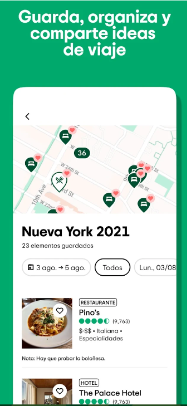
\includegraphics[width=0.32\textwidth]{img/tripadvisor.png} & 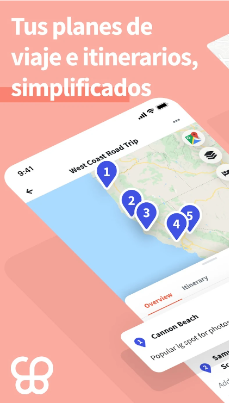
\includegraphics[width=0.34\textwidth]{img/wanderlog.png} \\
	\hline
	\href{https://play.google.com/store/apps/details?id=com.visitacity}{\textbf{Visit A City}} & \href{https://play.google.com/store/apps/details?id=com.tiqets.tiqetsapp}{\textbf{Tiqets - Museos y Atracciones}} \\
	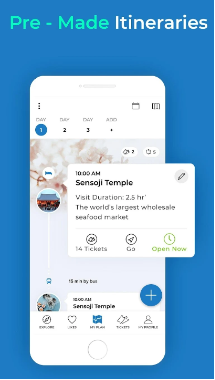
\includegraphics[width=0.35\textwidth]{img/visit_a_city.png} & 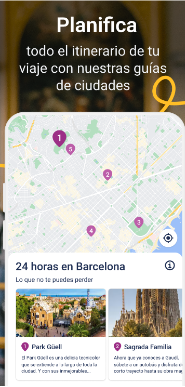
\includegraphics[width=0.31\textwidth]{img/tiquets.png} \\
	\hline
	\end{tabular}
	\caption{Aplicaciones Similares}
	\label{fig:apps_similares}
	\end{table}

\newpage

\begin{table}[h]
	\centering
	\renewcommand{\arraystretch}{1.5} % Controla el espaciado entre las líneas
	\rowcolors{2}{gray!20}{white} % Alterna colores de fondo en las filas
	\resizebox{\textwidth}{!}{ % Ajusta el tamaño de la tabla al ancho de la página
		\begin{tabular}{m{4cm} >{\centering\arraybackslash}m{2cm} >{\centering\arraybackslash}m{2cm} >{\centering\arraybackslash}m{2cm} >{\centering\arraybackslash}m{2cm} >{\centering\arraybackslash}m{2.5cm}} % Ajustamos los anchos de las columnas
			\toprule  
			\textbf{Característica} & \textbf{Tripadvisor} & \textbf{Wanderlog} & \textbf{Visit \newline A City} & \textbf{Tiquets} & \textbf{\textit{Eco City Tour}} \\
			\midrule
			Versión de pago & Sí & Sí & No & No & No\\
			Recomendaciones tienen en cuenta factores de sostenibilidad & No & No & No & No & Sí\\
			Modificación dinámica de rutas & Sí & No & No & No & Sí\\
			Intereses de terceros pueden afectar a los resultados & Sí & Sí & No & No & No \\
			Fuente de datos & Propia & Usuarios - LLM & Usuarios & Propia & LLM\\
			\bottomrule
		\end{tabular}
	}
	\caption{Comparación de aplicaciones similares}
	\label{herramientasportipodeuso}
\end{table}



	
\section{Otros \acrfull{tfg}}
	\subsection{Chatbot}
	Trabajo Fin de Carrera de José María Redondo Guerra \cite{chatbot_github} que tuvo como tutores a José Ignacio Santos Martín y Carlos López Nozal.
	
	Este trabajo fue desarrollado usando \acrfull{llm} para la generación de un chat con un sistema \acrshort{rag} para obtener la información de las normas de los \acrshort{tfg} y así mejorar sus respuestas.
	
	\subsection{Visualización de las actividades socioculturales en Castilla y León CULTURALCyL}
	Trabajo Fin de Carrera de Yanela Lozano Pérez con tutores José Ignacio Santos, Virginia Ahedo y Silvia Díaz.
	Esta aplicación mostraba información de eventos culturales para lo cual usaba una aplicación móvil con servicios API.
	Es especialmente interesante como ejemplo de una aplicación móvil con una fuerte característica de usabilidad, ya que se centra en la visualización de mucha información que debe recibir el usuario de manera clara y sencilla.
\capitulo{7}{Conclusiones y Líneas de trabajo futuras}
\section*{Conclusiones}
\section*{Líneas de trabajo futuras}
Existen múltiples maneras de expandir y llenar de nuevas funcionalidades a la aplicación llevada a cabo.
Por citar algunas que puedan resultar más útiles al usuario:
\begin{itemize}
    \item \textbf{Gamificación:} Recompensas por rutas completadas o distancia recorrida con un medio ecológico. Logros que desbloqueen aspectos visuales del icono de la aplicación.
    \item \textbf{Ratings:} Valorar las tours generados permitiendo la búsqueda de los mismos a otros usuarios.
    \item \textbf{Mejora en planificador de rutas:} Teniendo en cuenta otras fuentes de datos que mejoren la sostenibilidad de los tours como por ejemplo información satelital que determine las rutas en función de la zona de sombra.
    \item \textbf{Multiplataforma:} La aplicación podría beneficiarse de su adaptación a otras plataformas, donde se tendría que tener en cuenta principalmente los permisos de localización. Al utilizar Flutter esta adaptación se podría realizar sobre el mismo código base, facilitando en gran medida su consecución.
	\item \textbf{Reconocimiento de lugares (Landmark Recognition):} Firebase ofrece una función avanzada de reconocimiento de lugares \cite{firebase_mlkit_landmarks} que permitiría añadir una capa de personalización en la aplicación. Esta funcionalidad permitiría al usuario tomar una foto de uno de los \acrlong{pdi} visitados, y la aplicación podría identificar automáticamente el lugar y actualizar el estado de la ruta en tiempo real, indicando que se ha completado la visita. Esta mejora no solo facilitaría el seguimiento de la ruta, sino que también proporcionaría una experiencia de usuario más interactiva y dinámica.
	\item \textbf{Registro y autenticación de usuarios:} Para implementar algunas de las mejoras propuestas, es necesaria una gestión integral de usuarios. Actualmente, no existe un proceso de registro o autenticación, ya que es Cloud Firestore quien asigna un identificador único a cada usuario. Aunque esta gestión permite identificar los Eco City Tours generados por cada usuario, presenta limitaciones, como la pérdida de acceso a los tours al reinstalar la aplicación, debido a la asignación de un nuevo identificador. Además, los tours previos quedarían en la base de datos sin posibilidad de ser recuperados. Implementar un sistema de registro y autenticación una vez configurado Firebase sería una tarea relativamente sencilla, que incluiría generar una pantalla de registro y acceso, así como modificar la configuración de Cloud Firestore para incluir módulos de autenticación mediante servicios como correo electrónico o cuentas de Google.
\end{itemize}

\printnoidxglossary[type=\acronymtype]
\printnoidxglossary[]
%\printacronyms
%\printglossary
%\printnoidxglossary[type=\acronymtype]
%\printglossary[type=\acronymtype]
%\printglossary




\bibliographystyle{plain}
\bibliography{bibliografia}

\end{document}


Las referencias se incluyen en el texto usando cite~\cite{wiki:latex}. Para citar webs, artículos o libros~\cite{koza92}, si se desean citar más de uno en el mismo lugar~\cite{bortolot2005, koza92}.

\section{Listas de items}

Existen tres posibilidades:

\begin{itemize}
	\item primer item.
	\item segundo item.
\end{itemize}

\begin{enumerate}
	\item primer item.
	\item segundo item.
\end{enumerate}

\begin{description}
	\item[Primer item] más información sobre el primer item.
	\item[Segundo item] más información sobre el segundo item.
\end{description}

\begin{itemize}
	\item 
\end{itemize}

\section{Tablas}

Igualmente se pueden usar los comandos específicos de \LaTeX o bien usar alguno de los comandos de la plantilla.

\tablaSmall{Herramientas y tecnologías utilizadas en cada parte del proyecto}{l c c c c}{herramientasportipodeuso}
{ \multicolumn{1}{l}{Herramientas} & App AngularJS & API REST & BD & Memoria \\}{ 
	HTML5 & X & & &\\
	CSS3 & X & & &\\
	BOOTSTRAP & X & & &\\
	JavaScript & X & & &\\
	AngularJS & X & & &\\
	Bower & X & & &\\
	PHP & & X & &\\
	Karma + Jasmine & X & & &\\
	Slim framework & & X & &\\
	Idiorm & & X & &\\
	Composer & & X & &\\
	JSON & X & X & &\\
	PhpStorm & X & X & &\\
	MySQL & & & X &\\
	PhpMyAdmin & & & X &\\
	Git + BitBucket & X & X & X & X\\
	Mik\TeX{} & & & & X\\
	\TeX{}Maker & & & & X\\
	Astah & & & & X\\
	Balsamiq Mockups & X & & &\\
	VersionOne & X & X & X & X\\
} 
Algunos conceptos teóricos de \LaTeX{} \footnote{Créditos a los proyectos de Álvaro López Cantero: Configurador de Presupuestos y Roberto Izquierdo Amo: PLQuiz}.
